% This LaTeX document needs to be compiled with XeLaTeX.
\documentclass[10pt]{article}
\usepackage[utf8]{inputenc}
\usepackage{ucharclasses}
\usepackage{graphicx}
\usepackage[export]{adjustbox}
\graphicspath{ {./images/} }
\usepackage{amsmath}
\usepackage{amsfonts}
\usepackage{amssymb}
\usepackage[version=4]{mhchem}
\usepackage{stmaryrd}
\usepackage{multirow}
\usepackage{polyglossia}
\usepackage{fontspec}
\usepackage{newunicodechar}
\setmainlanguage{english}
\setotherlanguages{hindi, hebrew}
\newfontfamily\hindifont{Noto Serif Devanagari}
\newfontfamily\hebrewfont{Noto Serif Hebrew}
\newfontfamily\lgcfont{CMU Serif}
\setDefaultTransitions{\lgcfont}{}
\setTransitionsFor{Hindi}{\hindifont}{\lgcfont}
\setTransitionsFor{Hebrew}{\hebrewfont}{\lgcfont}

\newunicodechar{×}{\ifmmode\times\else{$\times$}\fi}

\begin{document}
Computer Engineering

\section*{Hardware}
\begin{itemize}
  \item CPU Central Processing Unit
  \item Memory Stores instructions and data
  \item Input / Output Interface to external devices
  \item System-Bus Electrical connection of blocks\\
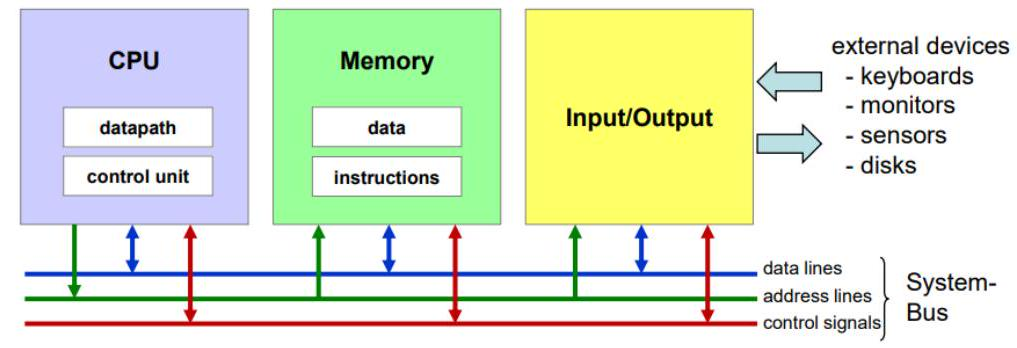
\includegraphics[width=\linewidth]{images/2024_12_29_79e6b22f503fb7b4f718g-01(1)}
\end{itemize}

\section*{Datapath}
\begin{itemize}
  \item ALU
  \item Registers
\end{itemize}

Arithmetic and Logic Unit Fast but limited storage inside CPU

Control Unit

\begin{itemize}
  \item Finite State Machine
\end{itemize}

Reads and executes instructions

\begin{itemize}
  \item Types of instructions Data transfer, Arithemtic, logical and jumps
\end{itemize}

\section*{Software}
\section*{From C to executable}
\begin{center}
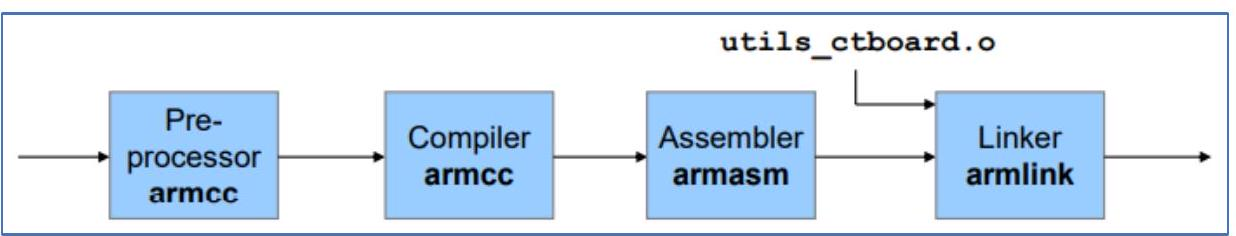
\includegraphics[width=\linewidth]{images/2024_12_29_79e6b22f503fb7b4f718g-01}
\end{center}

\begin{enumerate}
  \item Preprocessor
\end{enumerate}

\begin{itemize}
  \item Text processing
  \item Pasting of \#include files
  \item Replacing macros (\#define)
\end{itemize}

\begin{enumerate}
  \setcounter{enumi}{1}
  \item Compiler
\end{enumerate}

\begin{itemize}
  \item Translate CPU-independent C-code into CPU-specific assembly code
\end{itemize}

\begin{enumerate}
  \setcounter{enumi}{2}
  \item Assembler
\end{enumerate}

\begin{itemize}
  \item Translate to machine instructions
  \item Result: Relocatable object file
  \item Binary file $\rightarrow$ not readable with text editor
\end{itemize}

\begin{enumerate}
  \setcounter{enumi}{3}
  \item Linker
\end{enumerate}

\begin{itemize}
  \item Merge object files
  \item Resolve dependencies and cross-references
  \item Create executable
\end{itemize}

\section*{Registers}
\begin{itemize}
  \item 16 Core Registers
  \item 32-Bit wide
  \item RO-R7 Lower Registers
  \item R8 - R12 Higher Registers
  \item R13 Stack Pointer Temp Storage
  \item R14 Link Register Return from Procs
  \item R15 Program Counter Addr of next Instr.
\end{itemize}

\section*{ALU}
\begin{itemize}
  \item 32-Bit wide processing unit
\end{itemize}

\section*{APSR (Flag Register)}
\begin{itemize}
  \item N Negative
  \item Z Zero
  \item C Carry
  \item V Overflow
\end{itemize}

\section*{Instruction Set}
\begin{center}
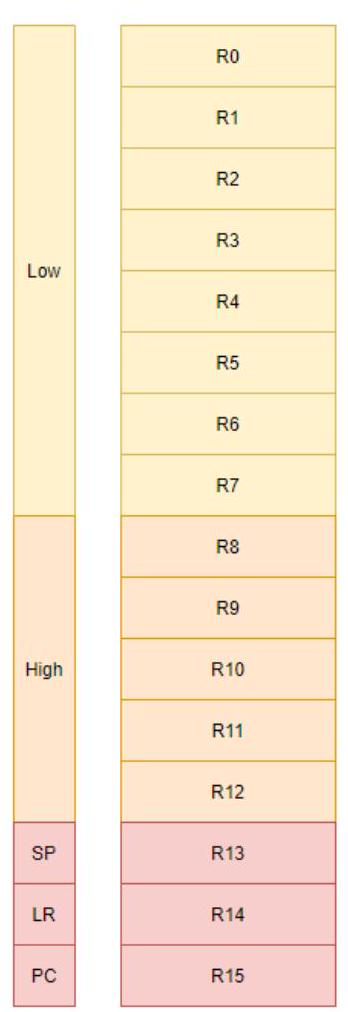
\includegraphics[width=\linewidth]{images/2024_12_29_79e6b22f503fb7b4f718g-02}
\end{center}

\begin{itemize}
  \item 16-Bit Thumb instruction encoding
\end{itemize}

\begin{center}
\begin{tabular}{llll}
Label & Instr. & Operands & Comments \\
\hline
demoprg & MOVS & R0,\#0xA5 & ; copy 0xA5 into register R0 \\
 & MOVS & R1,\#0x11 & ; copy 0x11 into register R1 \\
 & ADDS & R0,R0,R1 & ; add contents of RO and R1 \\
\end{tabular}
\end{center}

\section*{Instruction Types}
\begin{itemize}
  \item Data transfer
  \item Data processing
  \item Control flow Move, Load and Store\\
Arithmetic, Logical and Shift operations\\
Branches and functions
\end{itemize}

\section*{Assembly Program Structure}
\begin{center}
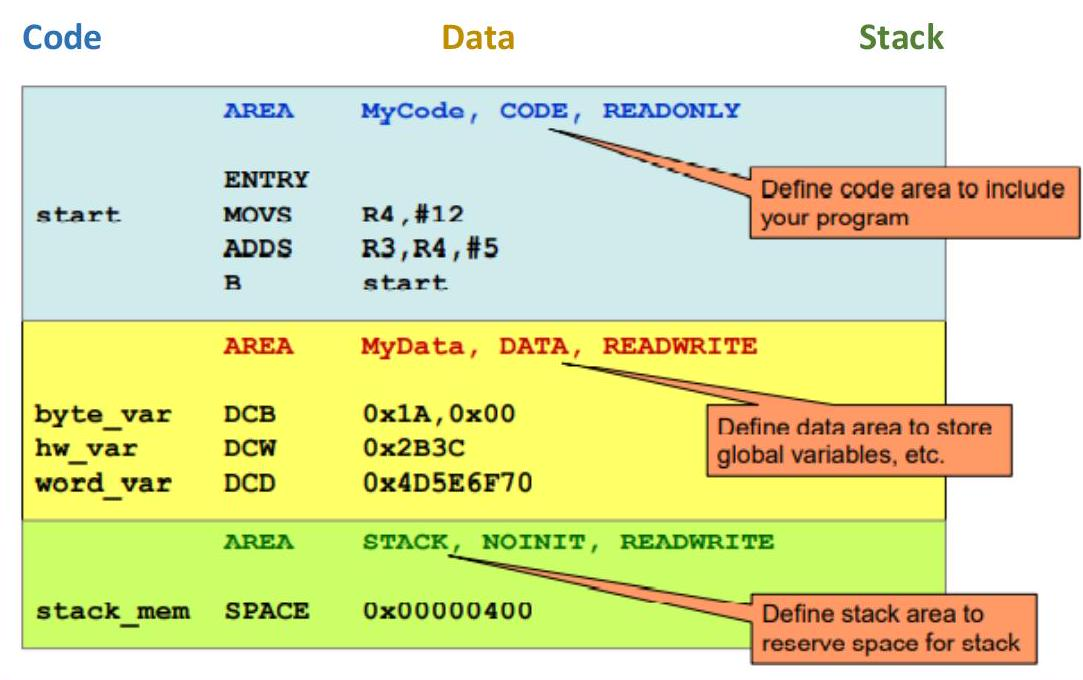
\includegraphics[width=\linewidth]{images/2024_12_29_79e6b22f503fb7b4f718g-02(1)}
\end{center}

Directives for initialized data

\begin{itemize}
  \item DCB Bytes
  \item DCW Half-Words
  \item DCD Words
\end{itemize}

\begin{center}
\begin{tabular}{|c|c|c|c|c|c|}
\hline
var1 & DCB & 0x1A &  &  &  \\
\hline
var2 & DCB & 0x2B & 0x3C & 0×4D & 0x5E \\
\hline
var3 & DCW & \multicolumn{2}{|r|}{0x6F70} & \multicolumn{2}{|c|}{0x8192} \\
\hline
var4 & $D C D$ & \multicolumn{4}{|c|}{0xA3B4C5D6} \\
\hline
\end{tabular}
\end{center}

Directives for uninitialized data

\begin{itemize}
  \item SPACE Bytes to be reserved
\end{itemize}

Pascal Isliker

\section*{Data Transfer Instructions}
\section*{Loading Data}
\begin{itemize}
  \item MOVS
  \item Reg to Reg MOVS R1, R2
  \item 8-Bit Literal MOVS R1,\#0x1C
  \item Constant MOVS R1, \#MyConst
  \item LDR
  \item 32-Bit Literal LDR R1, \#OxA1B2C3D4
  \item Literal + Offset LDR R1, [PC, \#12]
  \item Constant LDR R1, =MyConst
  \item Reg Value LDR R1, [R2]
  \item LDRB
  \item Load Register Byte
  \item Bits 31 to 8 set to zero
  \item LDRH
  \item Load Register Half-word
  \item Bits 31 to 16 set to zero
\end{itemize}

\section*{Load Array}
\begin{itemize}
  \item my\_array $=3$ * 4 Bytes
  \item Instructions $=5$ * 2 Bytes
  \item Literals (0x08) $=1 * 4$ Bytes\\
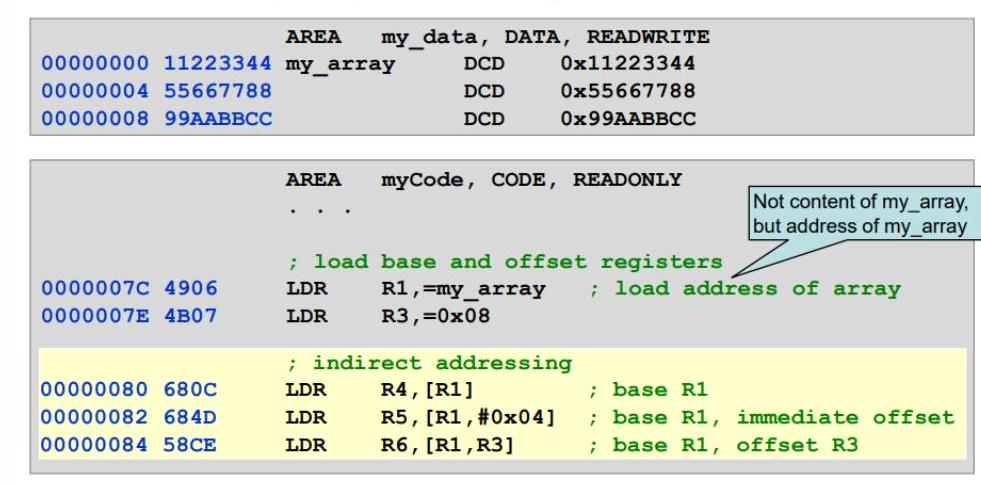
\includegraphics[width=\linewidth]{images/2024_12_29_79e6b22f503fb7b4f718g-03(1)}\\
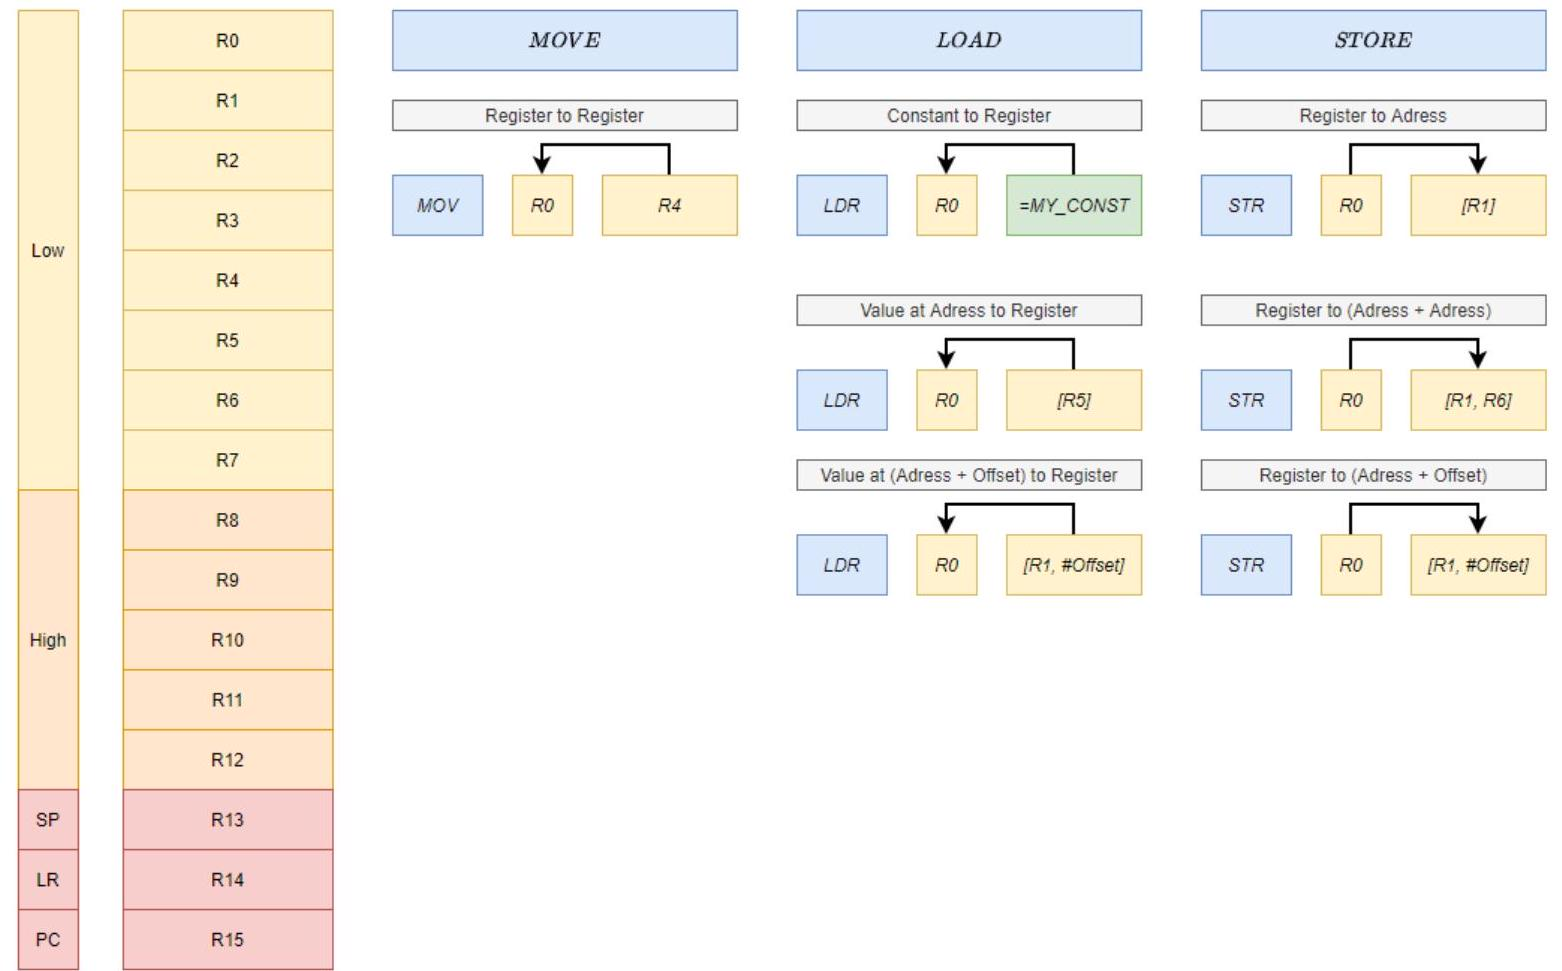
\includegraphics[width=\linewidth]{images/2024_12_29_79e6b22f503fb7b4f718g-03}
\end{itemize}

Storing Data

\begin{itemize}
  \item STR
  \item Value from Register STR R1, [R2]
  \item Value from Reg + Offset $S T R R 1,[R 2, \# 0 x 04]$
  \item STRB
  \item Store Register Byte (Low 8 bits of register stored)
  \item STRH
  \item Store Register Half-word (Low 15 bits of register stored)
\end{itemize}

\section*{Arithmetic Operations}
Flags (APSR = N, Z, C, V)\\
Instructions ending with with «S» allow flag modification

\begin{itemize}
  \item ADDS
  \item SUBS
  \item MOVS
  \item LSLS
\end{itemize}

\begin{center}
\begin{tabular}{|llll|}
\hline
Flag & Meaning & Action & Operands \\
\hline
Negative & MSB =1 & $\mathrm{N}=1$ & signed \\
Zero & Result $=0$ & $\mathrm{Z}=1$ & signed, unsigned \\
Carry & Carry & $\mathrm{C}=1$ & unsigned \\
Overflow & Overflow & $\mathrm{V}=1$ & signed \\
\hline
\end{tabular}
\end{center}

\section*{Overview}
\begin{itemize}
  \item ADD / ADDS
  \item ADCS Addition with Carry
  \item ADR Address to Register
  \item SUB / SUBS
  \item SBCS
  \item RSBS
  \item MULS
\end{itemize}

Subtraction\\
Subtraction with carry (borrow)\\
Reverse Subtract (negative)\\
Multiplication\\
$A+B$\\
$A+B+c$\\
$P C+A$\\
$A-B$\\
$A-B-!c$\\
$-1 \cdot A$\\
$A \cdot B$

Multi-Word Addition with ADCS\\
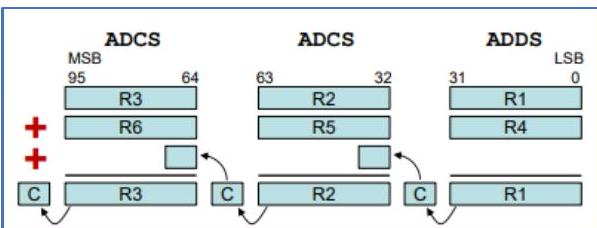
\includegraphics[width=\linewidth]{images/2024_12_29_79e6b22f503fb7b4f718g-04}

\begin{center}
\begin{tabular}{|c|c|c|c|}
\hline
ADDS & R1, & R1, & R4 \\
\hline
ADCS & R2, & R2, & R5 \\
\hline
ADCS & R3, & R3, & R6 \\
\hline
\end{tabular}
\end{center}

Multi-Word Subtraction with SBCS\\
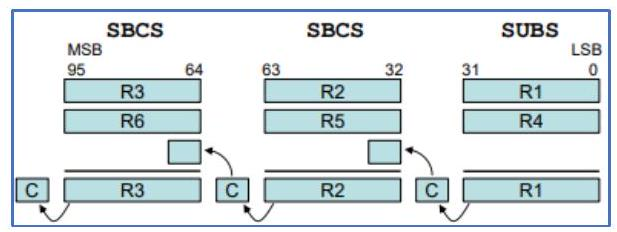
\includegraphics[width=\linewidth]{images/2024_12_29_79e6b22f503fb7b4f718g-04(1)}

\begin{center}
\begin{tabular}{|c|c|c|c|}
\hline
SUBS & R1, & R1, & R4 \\
\hline
SBCS & R2, & R2, & R5 \\
\hline
SBCS & R3, & R3, & R6 \\
\hline
\end{tabular}
\end{center}

\section*{Negative Number}
\begin{itemize}
  \item 2' Complement $\quad A=!A+1$
\end{itemize}

\section*{Carry and Overflow}
unsigned

\begin{itemize}
  \item Addition $\rightarrow \quad \mathrm{C}=1 \rightarrow$ carry result too large for available bits
  \item Subtraction $\rightarrow \mathrm{C}=0 \rightarrow$ borrow result less than zero $\rightarrow$ no negative numbers\\
signed
  \item Addition $\rightarrow \quad$ potential overflow in case of operands with equal signs
  \item Subtraction $\rightarrow$ potential overflow in case of operands with opposite signs
\end{itemize}

\section*{Addition and Subtraction}
\begin{itemize}
  \item Addition $\quad \mathrm{C}=1 \rightarrow$ Carry
\end{itemize}

\begin{center}
\begin{tabular}{|rrrrr|}
\hline
1 & 1 & 0 & 1 & $13 d$ \\
0 & 1 & 1 & 1 & $7 d$ \\
1 & 1 & 1 & 1 &  \\
1 &  &  &  &  \\
1 & 0 & 1 & 0 & 0 \\
\end{tabular}
\end{center}

\begin{itemize}
  \item Subtraction $\quad \mathrm{C}=0 \rightarrow$ Borrow sign\\
$6 d-14 d=0110 b-1110 b=0110 b+0010 b$
\end{itemize}

$$
\begin{array}{llllll}
0 & 1 & 1 & 0 & 6 d \\
0 & 0 & 1 & 0 & 2 d=\operatorname{TC}(14 d)
\end{array}
$$

0100\\
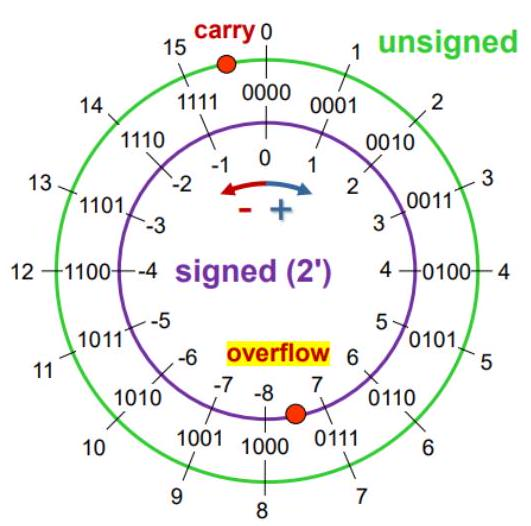
\includegraphics[width=\linewidth]{images/2024_12_29_79e6b22f503fb7b4f718g-04(2)}

\section*{Branch Instructions}
\begin{center}
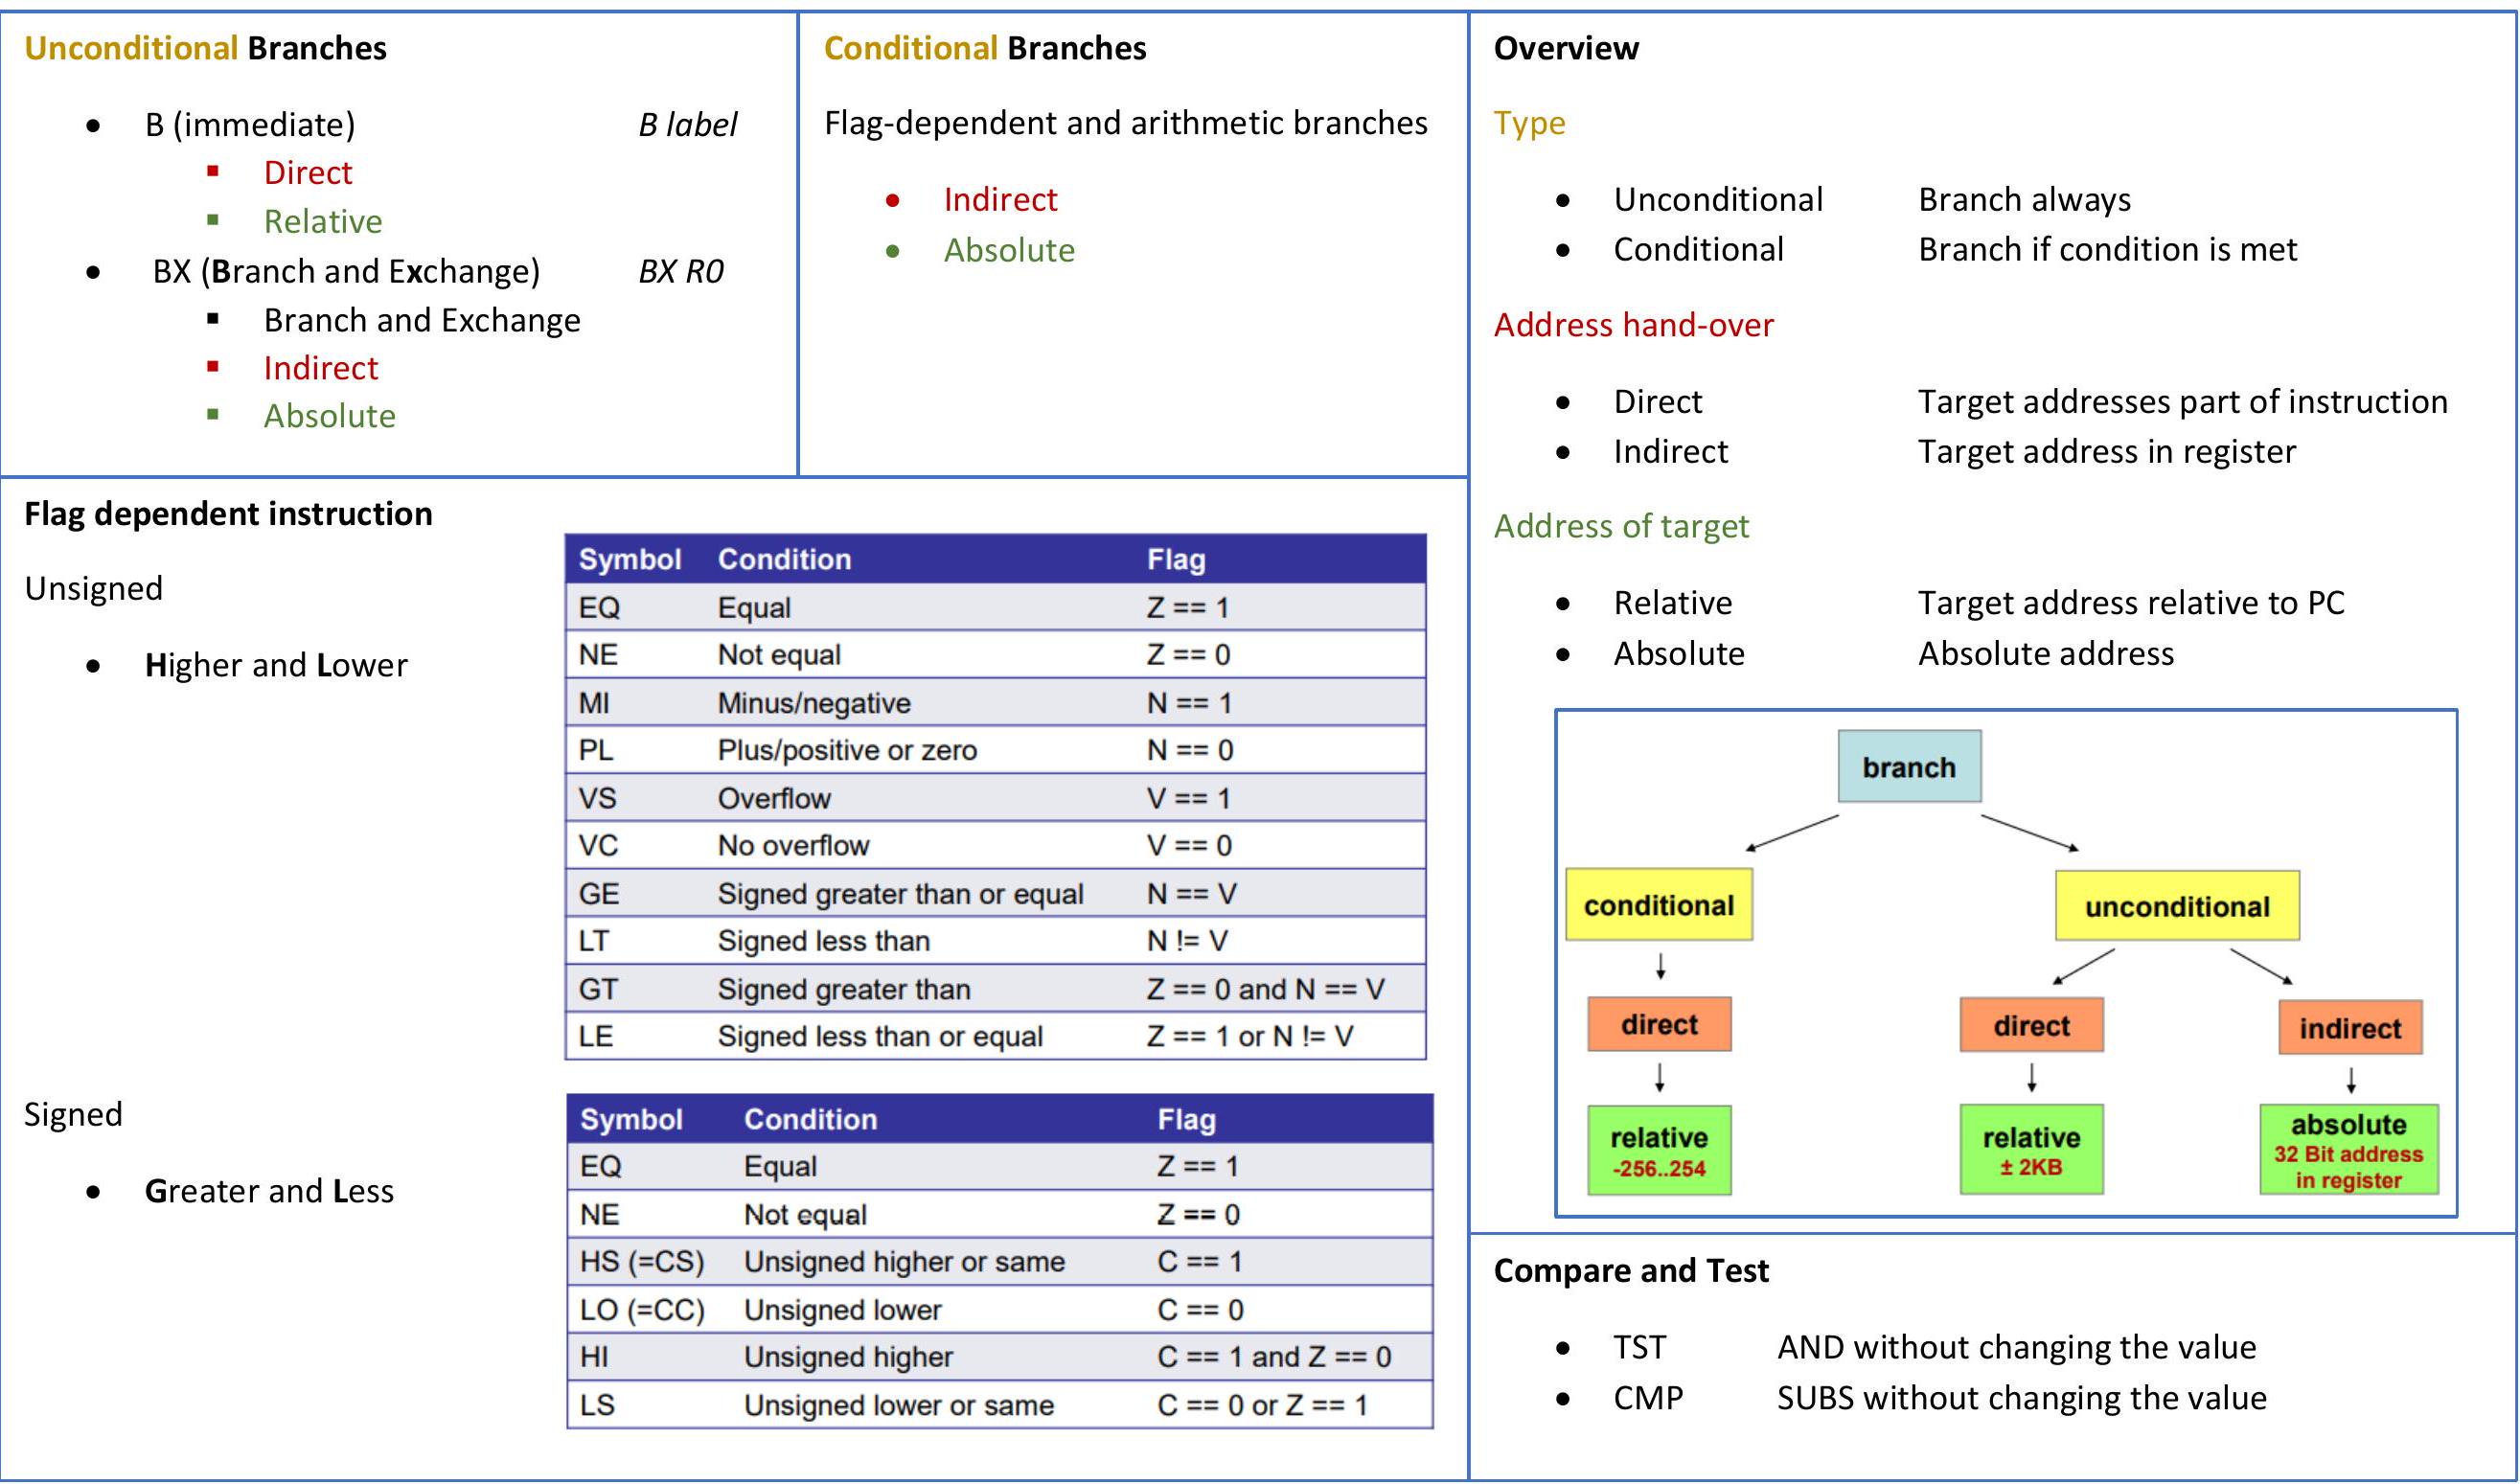
\includegraphics[width=\linewidth]{images/2024_12_29_79e6b22f503fb7b4f718g-05}
\end{center}

\section*{Logical Instructions}
The following instruction only affect N and Z flags

\begin{itemize}
  \item ANDS
  \item BICS
  \item EORS
  \item MVNS Bitwise NOT
  \item ORRS
\end{itemize}

Bitwise OR

Rdn \# Rm\\
Rdn \& Rm\\
Rdn \& ! Rm $\quad a \& \sim b$\\
Rdn \$ Rm $\quad a{ }^{\wedge} b$\\
Rm a\\
a | b

Shift Instructions

\begin{itemize}
  \item LSLS Logical Shift Left $\quad 2^{n} \cdot R n \quad 0 \rightarrow L S B$
  \item LSRS Logical Shift Right $\quad 2^{-n} \cdot R n \quad 0 \rightarrow M S B$
  \item ASRS Arithmetic Shift Right $\quad R^{-n} \pm \pm M S B \rightarrow M S B$
  \item RORS Rotate Right $\quad L S B \rightarrow M S B$\\
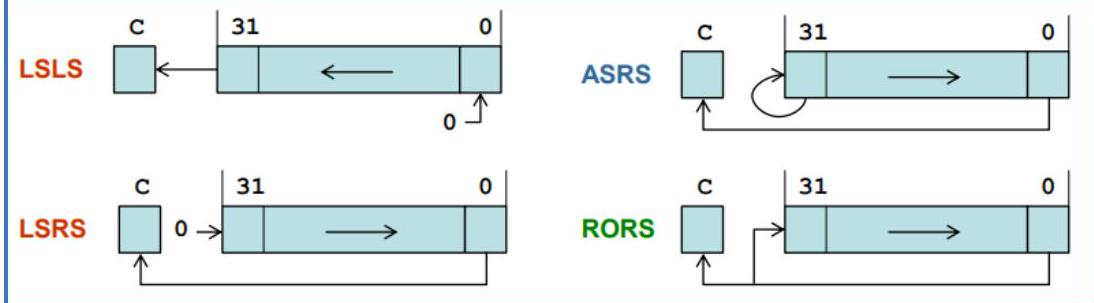
\includegraphics[width=\linewidth]{images/2024_12_29_79e6b22f503fb7b4f718g-06}
\end{itemize}

\section*{Sign-Extension}
Add additional bits

\begin{itemize}
  \item Unsigned zero extension fill left bits with zero
  \item Signed sign extension copy sign bit to the left
\end{itemize}

\begin{center}
\begin{tabular}{|c|c|c|c|c|}
\hline
\multicolumn{2}{|l|}{Unsigned $\rightarrow \boldsymbol{\sim}$ Zero Extension} &  & \multirow[b]{2}{*}{$\rightarrow$} & \multirow[b]{2}{*}{00000011} \\
\hline
$1011 \rightarrow$ & 00001011 & 0011 &  &  \\
\hline
\multicolumn{5}{|l|}{Signed $\boldsymbol{\rightarrow}$ Sign Extension} \\
\hline
$1011 \rightarrow$ & 11111011 & 0011 & $\rightarrow$ & 00000011 \\
\hline
\end{tabular}
\end{center}

\section*{Truncation}
Cast cuts out the left most digits

\begin{itemize}
  \item Signed possible change of sign
  \item Unsigned results in module operation
\end{itemize}

\section*{Integer ranges based on word sizes}
\begin{center}
\begin{tabular}{|c|c|c|c|c|c|c|c|}
\hline
\multirow[t]{6}{*}{8-bit} & \( \begin{gathered} \text { hex } \\ 0 \times 00 \end{gathered} \) & unsigned & signed & 16-bit & hex 0×0000 & unsigned & signed \\
\hline
 &  &  &  &  &  &  &  \\
\hline
 & 0x75 & 127 & 127 &  & 0x7FFF & F 32'767 & $32 \cdot 767$ \\
\hline
 & 0x80 & 128 & -128 &  & 0x8000 & $032 \cdot 768$ & -32'768 \\
\hline
 &  & . . . & -. &  & . . & . . &  \\
\hline
 & 0xFF & 255 & -1 &  & 0xFFFF & F 65'535 & -1 \\
\hline
\multicolumn{2}{|r|}{\multirow[t]{7}{*}{32-bit}} & \multicolumn{2}{|l|}{hex} & \multicolumn{2}{|l|}{unsigned} & signed &  \\
\hline
 &  & \multicolumn{2}{|l|}{0x0000 0000} & \multicolumn{2}{|l|}{o} & 0 &  \\
\hline
 &  & \multicolumn{2}{|l|}{\multirow[t]{2}{*}{0x7FFF'FFFF}} & \multicolumn{2}{|l|}{\multirow[t]{2}{*}{2'147'483'647}} & ... &  \\
\hline
 &  &  &  &  &  & 2'147'483' &  \\
\hline
 &  & \multicolumn{2}{|l|}{0x8000'0000} & \multicolumn{2}{|l|}{2'147'483'648 -} & -2'147'483' &  \\
\hline
 &  & \multicolumn{2}{|l|}{\multirow[t]{2}{*}{0xFFFF'FFFF}} & \multicolumn{2}{|l|}{\multirow[t]{2}{*}{4'294'967'295}} & -. &  \\
\hline
 &  &  &  &  &  & -1 &  \\
\hline
\end{tabular}
\end{center}

\begin{center}
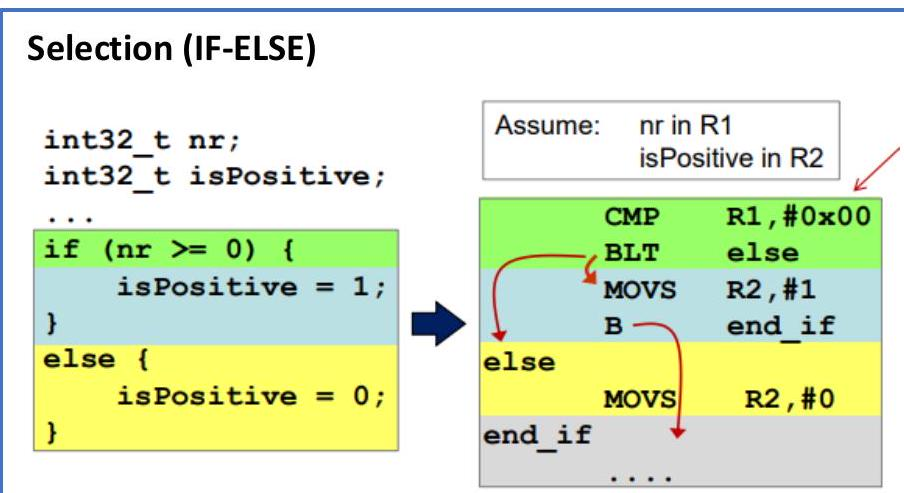
\includegraphics[width=\linewidth]{images/2024_12_29_79e6b22f503fb7b4f718g-07(3)}
\end{center}

\section*{Switch}
\section*{- Jump Table}
uint32\_t result, n; switch (n) 1\\
case 0:\\
result += 17; break;\\
case 1:\\
result += 13; //fall through\\
case 3: case 5 result += 37; break;\\
default:\\
result $=0$;\\
\}

\begin{center}
\begin{tabular}{|c|c|c|}
\hline
\multirow[t]{7}{*}{NR\_CASES case\_switch} & EQU & 6 \\
\hline
 & CMP & R1, \#NR\_CASES \\
\hline
 & BHS & case\_default \\
\hline
 & LSLS & R1, \#2 ; * 4 \\
\hline
 & LDR & R7, =jump\_table \\
\hline
 & LDR & R7, [R7, R1] \\
\hline
 & BX & R7 \\
\hline
case\_0 & ADDS & R2, R2, \#17 \\
\hline
case\_1 & ADDS & R2, R2, \#13 \\
\hline
\multirow[t]{2}{*}{case\_3\_5} & ADDS & R2, R2, \#37 \\
\hline
 & B & end\_sw\_case \\
\hline
case\_default & Movs & R2,\#0 \\
\hline
end\_sw\_case & ... &  \\
\hline
\multirow[t]{6}{*}{jump\_table} & DCD & case\_0 \\
\hline
 & DCD & case\_1 \\
\hline
 & DCD & case\_default \\
\hline
 & DCD & case\_3\_5 \\
\hline
 & DCD & case\_default \\
\hline
 & DCD & case\_3\_5 \\
\hline
\end{tabular}
\end{center}

\section*{Loops}
\begin{itemize}
  \item Do while: Post-Test Loop\\
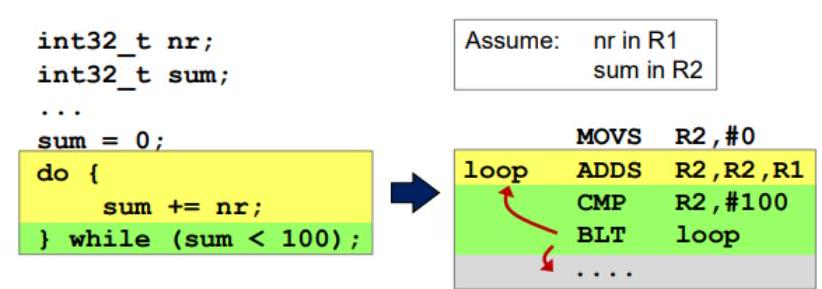
\includegraphics[width=\linewidth]{images/2024_12_29_79e6b22f503fb7b4f718g-07}
  \item While = Pre-Test Loop\\
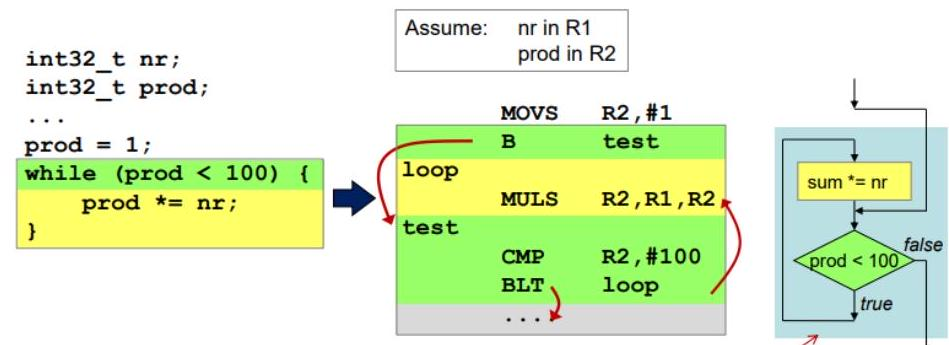
\includegraphics[width=\linewidth]{images/2024_12_29_79e6b22f503fb7b4f718g-07(1)}
  \item For = Pre-Test Loop\\
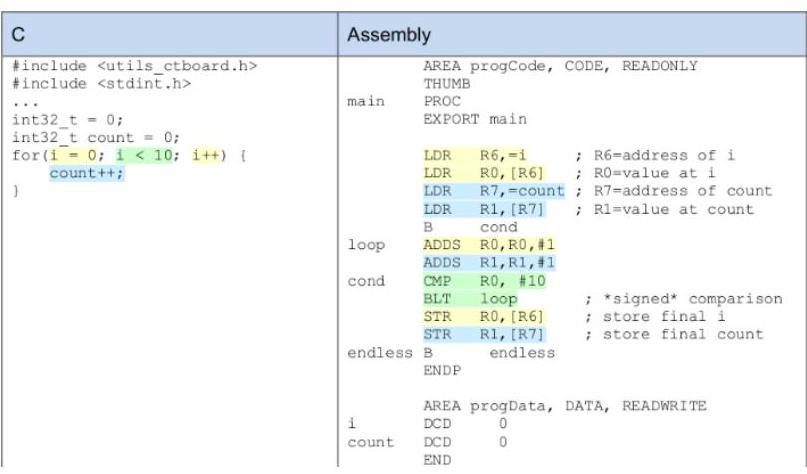
\includegraphics[width=\linewidth]{images/2024_12_29_79e6b22f503fb7b4f718g-07(2)}
\end{itemize}

\section*{Subroutine Call and Return}
\begin{itemize}
  \item Label with Name (MulBy3)
  \item Return Statement (BX $1 R$ )
\end{itemize}

\begin{center}
\begin{tabular}{lllll}
00000050 & 4604 & MulBy3 & MOV & R4,R0 \\
00000052 & 0040 & LSLS & RO, \#1 &  \\
00000054 & 4420 & ADD & R0,R4 &  \\
00000056 & 4770 & BX & LR &  \\
\hline
\end{tabular}
\end{center}

Stack

\begin{itemize}
  \item Stack Area (Section)
  \item Stack Pointer (SP)
  \item PUSH \{...\}
  \item POP \{...\}
  \item Direction on ARM
  \item Alignment
  \item Only words
\end{itemize}

Continuous area of RAM\\
R13 $\rightarrow$ points to last written data value\\
Decrement SP and store words\\
Read words and increment SP\\
full-descending stack\\
word-aligned\\
32-Bit

\section*{Stack - Push and Pop}
\begin{itemize}
  \item Number of Pushs = Number of Pops
  \item Stack-limit < SP < stack-base\\
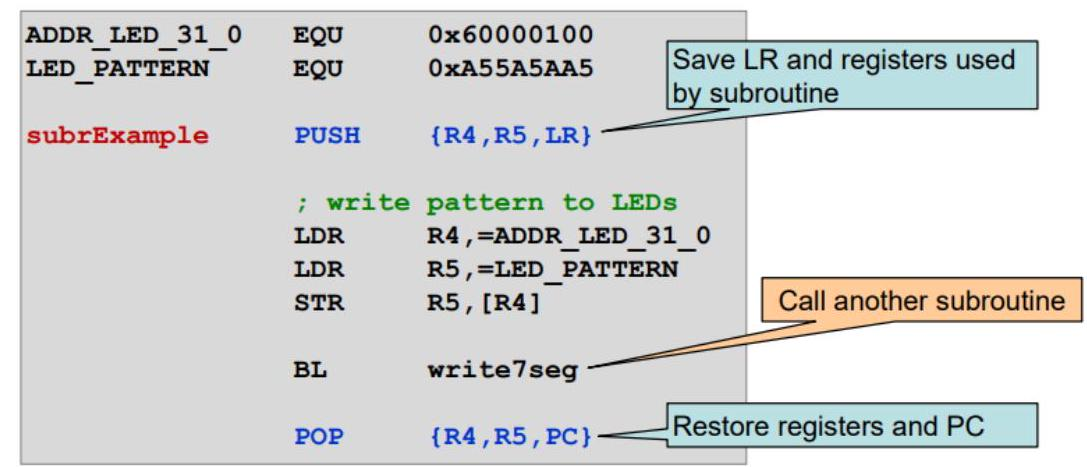
\includegraphics[width=\linewidth]{images/2024_12_29_79e6b22f503fb7b4f718g-08}
\end{itemize}

PUSH \{R2,R3,R6\}

\begin{center}
\begin{tabular}{llll}
00000000 & B083 & SUB & SP,SP,\#12 \\
00000002 9200 & STR & R2,[SP] &  \\
00000004 & 9301 & STR & R3,[SP,\#4] \\
000000069602 & STR & R6,[SP,\#8] &  \\
\end{tabular}
\end{center}

\section*{POP \{R2,R3,R6\}}
\begin{center}
\begin{tabular}{|llll|}
\hline
00000008 9A00 & LDR & R2,[SP] \\
0000000A 9B01 & LDR & R3,[SP,\#4] \\
0000000C 9B02 & LDR & R6,[SP,\#8] \\
0000000E B003 & ADD & SP,SP,\#12 \\
\hline
\end{tabular}
\end{center}

\section*{Where}
\begin{itemize}
  \item Register
  \item Global variables
  \item Stack
  \item Caller: PUSH parameter on stack
  \item Callee: Access parameter through LDR
\end{itemize}

\section*{Reentrancy}
\begin{itemize}
  \item Recursive Function Calls
  \item Registers and gobal variables are overwritten
  \item Requires an own set of data for each call
  \item Solution:
  \item ARM Procedure Call Standard
\end{itemize}

\section*{Passing through global variables}
\begin{itemize}
  \item Shared variables in data area
  \item Overhead to access variable
  \item Error prone, unmaintainable
  \item By reference
  \item Allows passing of larger structures
\end{itemize}

\section*{ARM Procedure call Standard}
\section*{Parameters}
\begin{itemize}
  \item Caller copies arguments From R0 to R3
  \item Caller copies additional parameters to stack
\end{itemize}

Returning fundamental data types

\begin{itemize}
  \item Smaller than word
  \item Word
  \item Double word
  \item 128-Bit\\
zero or sign extend to word return in RO return in RO / R1 return in RO - R3
\end{itemize}

Returning composite data types

\begin{itemize}
  \item Up to 4 bytes\\
return in RO
  \item Larger than 4 bytes stored in data area\\
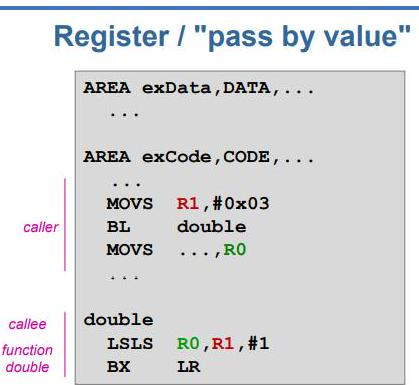
\includegraphics[width=\linewidth]{images/2024_12_29_79e6b22f503fb7b4f718g-09(2)}
\end{itemize}

Register Usage

\begin{center}
\begin{tabular}{|c|c|c|}
\hline
Register & Synonym & Role \\
\hline
ro & a1 & Argument / result / scratch register 1 \\
\hline
r1 & a2 & Argument / result / scratch register 2 \\
\hline
I2 & a3 & Argument / scratch register 3 \\
\hline
r3 & a4 & Argument / scratch register 4 \\
\hline
ז4 & v1 & Variable register 1 \\
\hline
r5 & v2 & Variable register 2 \\
\hline
r6 & v3 & Variable register 3 \\
\hline
r7 & v4 & Variable register 4 \\
\hline
ז8 & v5 & Variable register 5 \\
\hline
r9 & v6 & 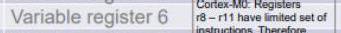
\includegraphics[width=\linewidth]{images/2024_12_29_79e6b22f503fb7b4f718g-09}
 \\
\hline
r10 & v7 & 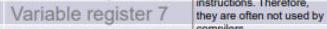
\includegraphics[width=\linewidth]{images/2024_12_29_79e6b22f503fb7b4f718g-09(1)}
 \\
\hline
r11 & v8 & Variable register 8 \\
\hline
r12 & IP & Intra-Procedure-call scratch register1) \\
\hline
r13 & SP &  \\
\hline
r14 & LR &  \\
\hline
\end{tabular}
\end{center}

Register contents\\
might be modified\\
might be modified

Callee must preserve contents\\
of these registers (Callee saved)\\
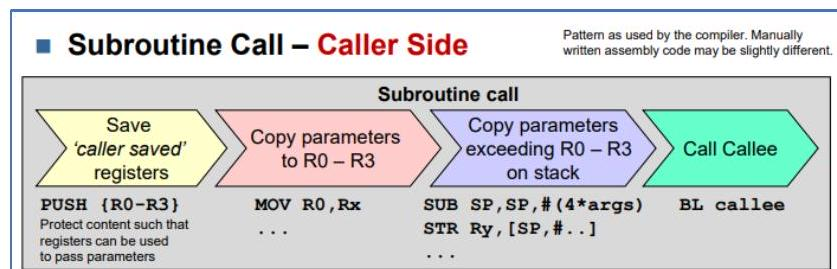
\includegraphics[width=\linewidth]{images/2024_12_29_79e6b22f503fb7b4f718g-09(3)}

On return from subroutine

\section*{Modular Coding / Linking}
\section*{From source code to executable program}
Compile / assemble each module

\begin{itemize}
  \item Results in an object file for each module
\end{itemize}

Link all object files

\begin{itemize}
  \item Results in one executable file\\
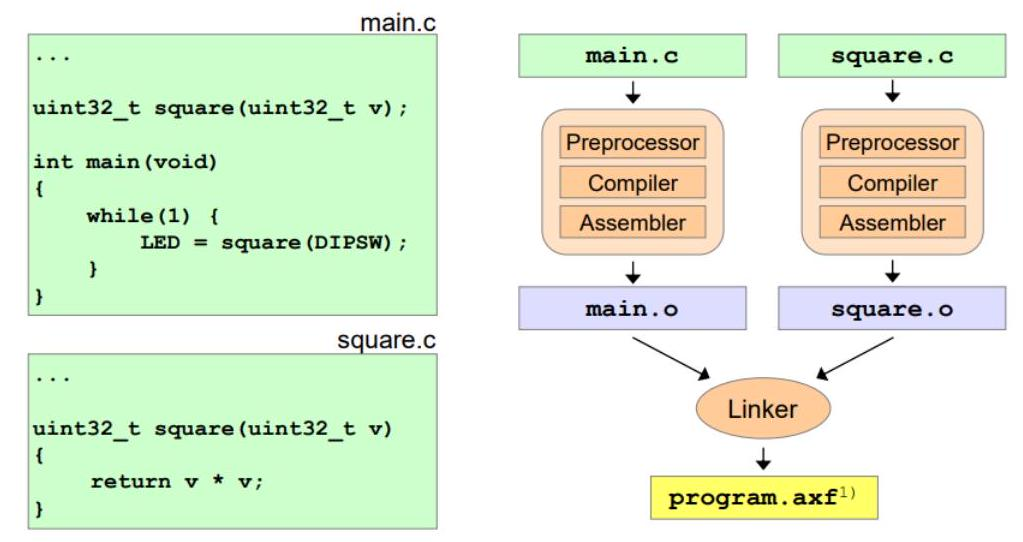
\includegraphics[width=\linewidth]{images/2024_12_29_79e6b22f503fb7b4f718g-10(2)}
\end{itemize}

\section*{Managing complexity by modular programming}
\begin{center}
\begin{tabular}{|l|l|}
\hline
Topic & Benefits \\
\hline
Enable working in teams & \begin{tabular}{l}
Multiple developers working on the same source \\
repository \\
\end{tabular} \\
\hline
Useful partitioning and structuring of the programs & Eases reuseing of modules \\
\hline
Individual verification of each module & Benefits all users of the module \\
\hline
Providing libraries of types and functions & For reuse instead of reinvention \\
\hline
\begin{tabular}{l}
Mixing of modules that are programmed in various \\
languages \\
\end{tabular} & E.g. mix C and assembly language modules \\
\hline
Only compile the changed modules & Speeds up compilation time \\
\hline
\end{tabular}
\end{center}

\section*{ARM assembly IMPORT and EXPORT keywords}
Linkage control

\begin{itemize}
  \item EXPORT for use by other module
  \item IMPORT from another module for use in this module Internal symbols
  \item Neither IMPORT nor EXPORT\\
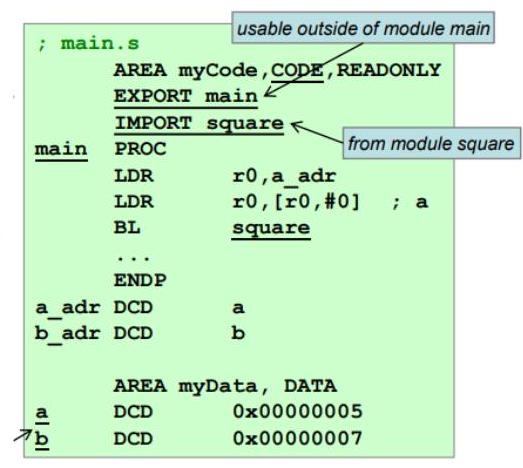
\includegraphics[width=\linewidth]{images/2024_12_29_79e6b22f503fb7b4f718g-10(1)}
\end{itemize}

\section*{Linker Input - Object files}
Code section Code and constant data of the module, base at address $0 \times 0$\\
Data section All global variables of the module, based at address $0 \times 0$\\
Symbol table All symbols with their attributes like global/local, reference\\
Relocation table

\begin{itemize}
  \item Which bytes oft he data and code section need to be adjusted (and how) after merging the sections in the linking process
\end{itemize}

ARM tool chain uses ELF for object files

\section*{Linker tasks}
\begin{itemize}
  \item Merge object file code sections
  \item Merge object file data sections
  \item Symbol resolution
  \item Address relocation
\end{itemize}

\section*{Linker Output}
\begin{itemize}
  \item $\quad$ AXF $=\mathbf{A R M}$ eXecutable File\\
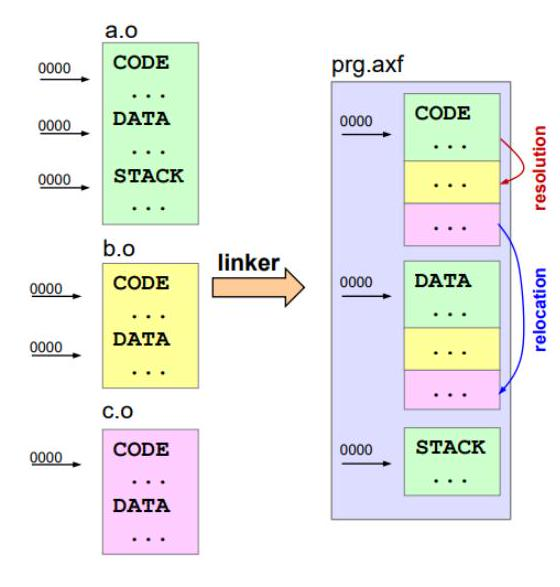
\includegraphics[width=\linewidth]{images/2024_12_29_79e6b22f503fb7b4f718g-10}
\end{itemize}

\section*{Interrupt sources}
\begin{itemize}
  \item Perfipherals signal to CPU that an event needs immediate attention
  \item Can alternativly be generated by software request
  \item Asynchronous to instruction execution
\end{itemize}

\section*{System exceptions}
\begin{itemize}
  \item Reset
  \item NMI
  \item Faults
  \item System Level Calls
\end{itemize}

Restart of processor\\
Non-maskable Interrupt (cannot be ignored) Undefined instructions OS calls - Instructions SVC and PendSV

\begin{center}
\begin{tabular}{|c|c|c|c|}
\hline
\multicolumn{3}{|l|}{\begin{tabular}{l}
PRIMASK \\
- Single bit controlling all maskable interrupts \\
\end{tabular}} & 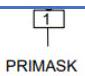
\includegraphics[width=\linewidth]{images/2024_12_29_79e6b22f503fb7b4f718g-11}
 \\
\hline
\begin{tabular}{l}
- Disable \\
- Enable \\
\end{tabular} & set PRIMASK clear PRIMASK & \begin{tabular}{l}
Assembly \\
CPSID ${ }^{1)}$ CPSIE ${ }^{1)}$ \\
\end{tabular} & C disable\_irq(); - enable\_irq(); \\
\hline
\multicolumn{4}{|l|}{On reset PRIMASK $=0 \quad \rightarrow$ enabled} \\
\hline
\end{tabular}
\end{center}

\section*{Storing the context}
Interrupt event can take place at any time

\begin{itemize}
  \item E.g. between TST and BEQ instructions
  \item ISR call requires automatic save off lags and caller saved registers
\end{itemize}

ISR call

\begin{itemize}
  \item Stores xPSR, PC, LR, R12, R0-R3 on Stack
  \item Stores EXC\_RETURN to LR
\end{itemize}

ISR Return

\begin{itemize}
  \item Use BX LR or POP \{..., PC\}
  \item Loading EXC Return into PC
  \item Restores RO-R3, R12, LR, PC and xPSR from Stack
\end{itemize}

\section*{Polling}
Periodic query of status information

\begin{itemize}
  \item Reading of status registers in loop
  \item Synchronous with main program
  \item Advantages
  \item Simple straightforward
  \item Implicit synchronisation
  \item Deterministic\\
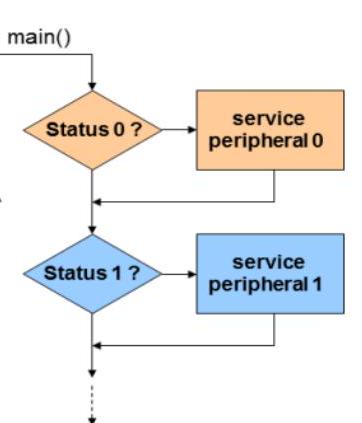
\includegraphics[width=\linewidth]{images/2024_12_29_79e6b22f503fb7b4f718g-11(1)}
  \item No additional interrupt logic required
  \item Disadvantages
  \item Busy wait -> wastes CPU time
  \item Reduced throughput
  \item Long reaction time
  \item No synchronization
  \item Difficult debugging\\
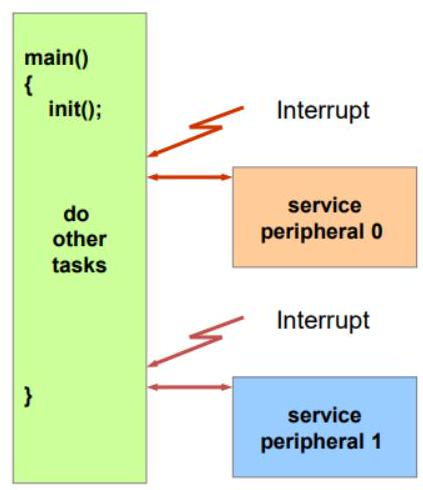
\includegraphics[width=\linewidth]{images/2024_12_29_79e6b22f503fb7b4f718g-11(2)}\\
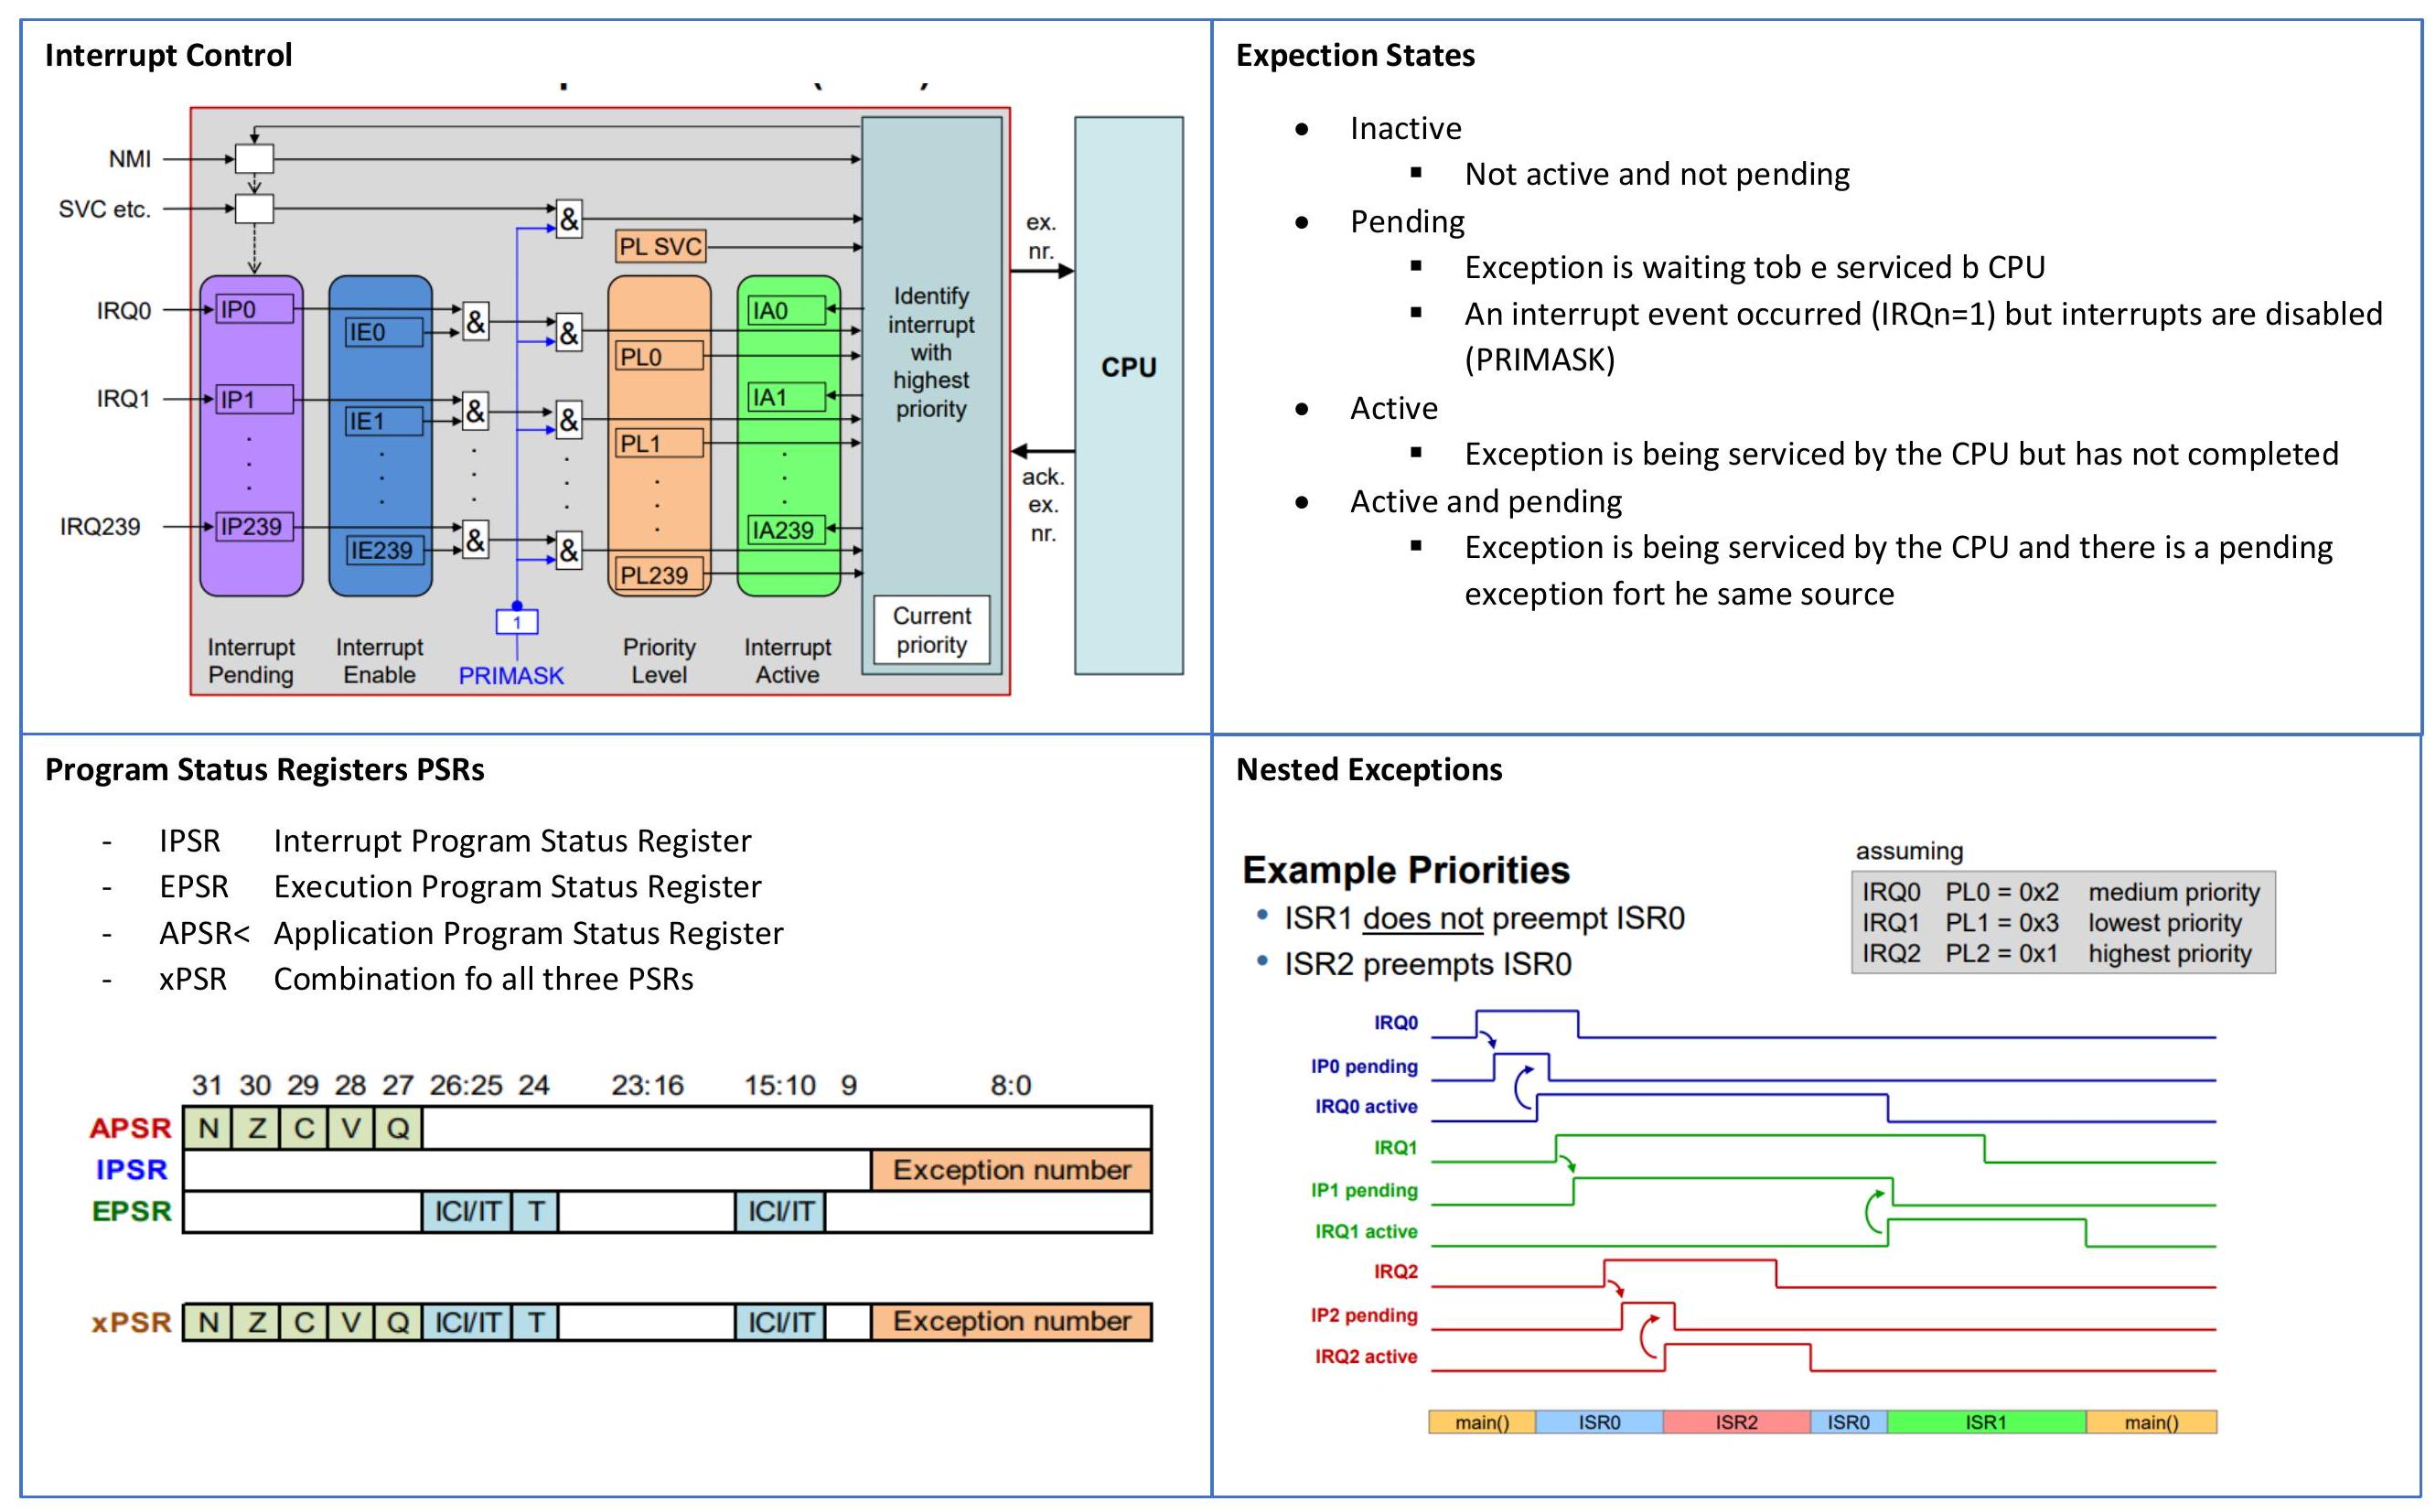
\includegraphics[width=\linewidth]{images/2024_12_29_79e6b22f503fb7b4f718g-12}
\end{itemize}

Improving System Performance

\begin{center}
\begin{tabular}{|l|l|}
\hline
Speed vs Low Power &  \\
Aspects of Optimization &  \\
\hline
Optimizing for & Drawbacks on \\
\hline
Higher speed & Power, cost, chip area \\
\hline
Lower cost & Speed, reliability \\
\hline
Zero power consumption & Speed, cost \\
\hline
Super reliable & Chip area, cost, speed \\
\hline
Temperature range & Power, cost lifetime \\
\hline
\end{tabular}
\end{center}

\section*{RISC = Reduced Instruction Set Computer}
\begin{itemize}
  \item Few instructions, unique instruction format
  \item Fast decoding, simple addressing
  \item Less hardware -> allows higher clock rates
  \item More chip space for registers (up to 256!)
  \item Load-store architecture reduces memory access,
\end{itemize}

CPU works at full-speed on registers

\begin{itemize}
  \item Higher clock frequencies
  \item Easy and shorter pipelines (instructio size / duration)\\
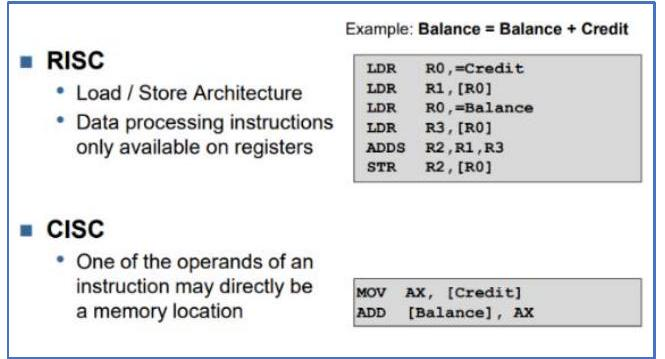
\includegraphics[width=\linewidth]{images/2024_12_29_79e6b22f503fb7b4f718g-13(1)}
\end{itemize}

CISC = Complex Instruction Set Computer

\begin{itemize}
  \item More complex and more instructions
  \item Less program memory needed with complex instructions
  \item Short programs may work faster with less memory accesses
\end{itemize}

\section*{Von Neuman Arhcitecture}
\begin{itemize}
  \item Same memory holds program and data
  \item $\quad$ Single bus system between CPU and memory Systembus\\
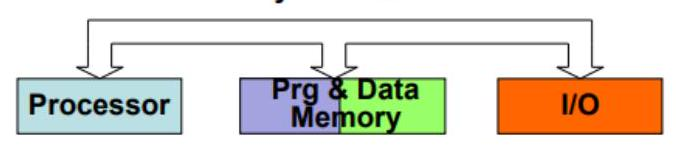
\includegraphics[width=\linewidth]{images/2024_12_29_79e6b22f503fb7b4f718g-13}
\end{itemize}

\section*{Harvard Architecture}
\begin{itemize}
  \item «Mark I» at Harvard University
  \item Separate memories for program and data
  \item Two sets of addresses/data buses between CPU and memory\\
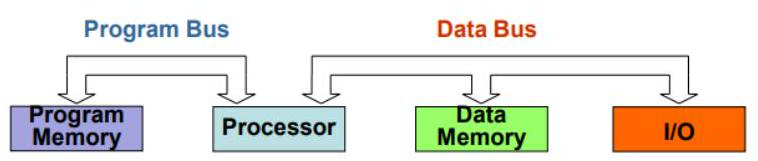
\includegraphics[width=\linewidth]{images/2024_12_29_79e6b22f503fb7b4f718g-13(2)}
\end{itemize}

How to Increase System Speed?\\
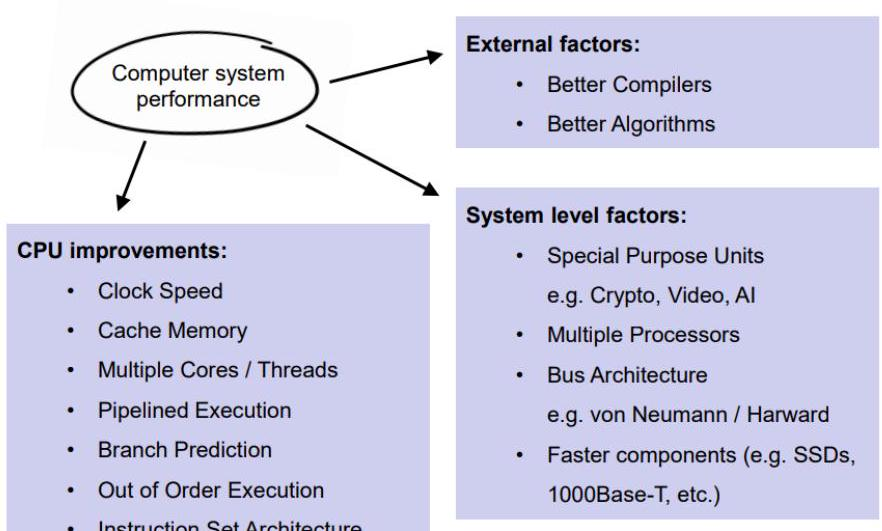
\includegraphics[width=\linewidth]{images/2024_12_29_79e6b22f503fb7b4f718g-13(3)}

Fetching the next instruction, while the current one decodes\\
Sequential vs. Pipelined\\
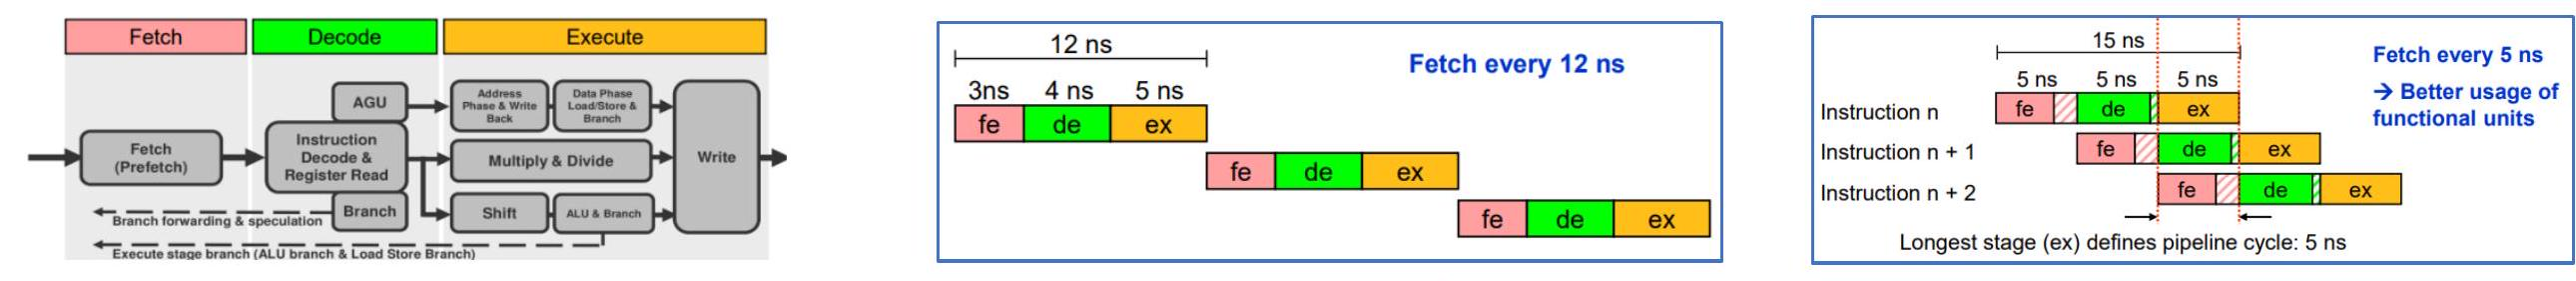
\includegraphics[width=\linewidth]{images/2024_12_29_79e6b22f503fb7b4f718g-14(2)}

\section*{Timings and definitions (Example)}
\begin{itemize}
  \item Fe: fetch Read instructions 3 ns
  \item De: decode Decode instruction, read register or memory 4 ns
  \item Ex: execute Execute instruction, write back result 5 ns\\
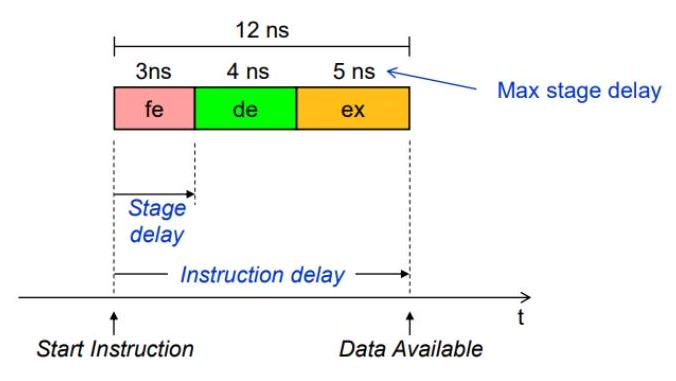
\includegraphics[width=\linewidth]{images/2024_12_29_79e6b22f503fb7b4f718g-14(1)}
\end{itemize}

\section*{Advantages of pipelining}
\begin{itemize}
  \item All stages are set tot he same execution time
  \item Massive performance gain
  \item Simpler hardware at each stage allows for a higher clock rate
\end{itemize}

\section*{Disadvantages}
\begin{itemize}
  \item A blocking stage blocks while pipeline
  \item Multiple stages may need to have access to the memory at the same time
\end{itemize}

\section*{Instructions per second}
Without pipelining

$$
\frac{\text { Instructions }}{\text { second }}=\frac{1}{\text { Instruction delay }}
$$

With pipelining

\begin{itemize}
  \item Pipeline needs to be filled first
  \item After filling, instructions are executed after every stage
\end{itemize}

$$
\frac{\text { Instructions }}{\text { second }}=\frac{1}{\text { Max stage delay }}
$$

\section*{Optimal pipelining}
\begin{itemize}
  \item All operations here are on registers
  \item In this example it takes 6 clock cycles to execute 6 instructions
  \item $\quad$ Clock cycles per instruction (CPI) = 1\\
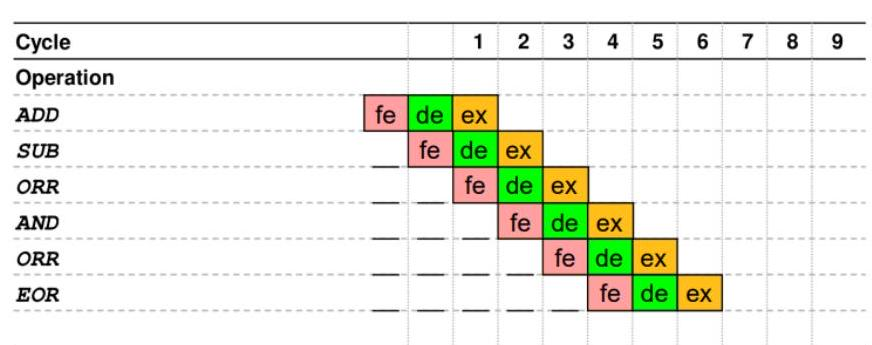
\includegraphics[width=\linewidth]{images/2024_12_29_79e6b22f503fb7b4f718g-14}
\end{itemize}

\section*{Special situation: LDR}
\begin{itemize}
  \item In this example it takes 7 clock cycles to execute 6 instructions
  \item Read cycle must complete on the bus before LDR instruction can complete
  \item Next 2 instructions must wait one pipeline cycle ( $\mathrm{S}=$ stall)
  \item Clock cycles per Instruction (CPI) $=1.2$
\end{itemize}

\section*{Control Hazards}
\begin{itemize}
  \item Branch / jump decisions occur in stage 3 (ex)
  \item Worst case scenario - conditional branch taken:\\
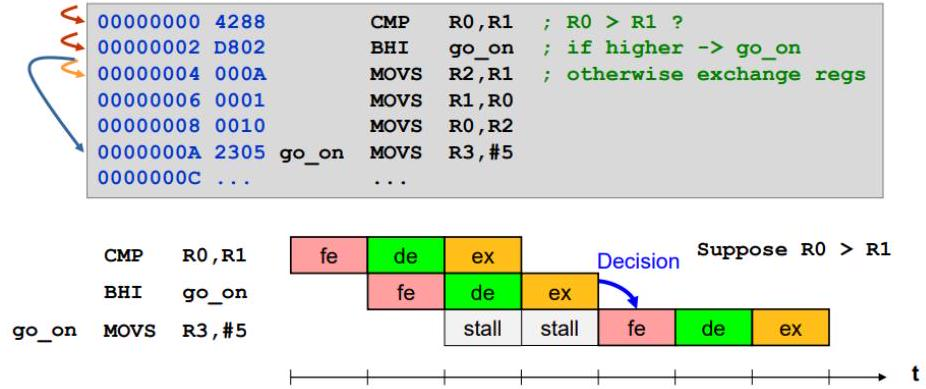
\includegraphics[width=\linewidth]{images/2024_12_29_79e6b22f503fb7b4f718g-15}
\end{itemize}

\section*{Reduce control hazards}
\begin{itemize}
  \item Loop fusion reduces control hazards
\end{itemize}

\section*{Ideas to further improve pipelining}
\begin{itemize}
  \item Branch prediction
  \item Store last decisions made for each conditional branch
  \item -> probability is high that the same decision is taken again
  \item Instruction prefetch
  \item Fetch several instructions in advance
  \item -> better use of system bus
  \item -> possibility of «Out of Order Execution»
  \item Out of Order Execution
  \item If one instruction stalls, it might be possible to already execute the next instruction
\end{itemize}

\section*{Limits of optimization}
\begin{itemize}
  \item Complex optimizations -> sever security problems
  \item Instructions executed, that would throw access violations under «In Order» circumstances.
  \item «Meltdown» and «Spectre» attacks: allow a process to access the data of another process
\end{itemize}

\section*{Parallel Computing}
\begin{itemize}
  \item Streaming / Vector processing One instruction processes multiple data items simultaneously
  \item Multithreading Multiple programs/threads share a single CPU
  \item Multicore Processors One processor contains multiple CPU cores
  \item Multiprocessor Systems A computer system contains multiple processors
\end{itemize}

\end{document}